% Phần BR5 và BR6 của Mục 5.4 (người phụ trách: Khang).
\subsection{BR05 -- Quản lý dựa trên dữ liệu}
\label{sec:5-eff-br05}

Bảng~\ref{tab:5-eff-br05} đối chiếu các tiêu chí chấp nhận của BR5 với bằng chứng thu được trên hệ thống chạy thật (dữ liệu từ bộ mô phỏng, qua Kafka, Spark, Iceberg, dbt và Trino). Mọi truy vấn trong mục này chạy bằng \code{just trino-sql}.

\begin{table}[H]
\centering
\caption{Tiêu chí chấp nhận của BR5 và bằng chứng}
\label{tab:5-eff-br05}
\small
\begin{tblr}{
  colspec = {X[2.2,l]X[3.4,l]X[0.9,c]}, rows = {abovesep=2pt, belowsep=2pt},
  hlines, vlines, row{1} = {font=\bfseries, bg=gray!20},
}
Tiêu chí chấp nhận & Bằng chứng & Kết quả \\
Tổng hợp gold khớp với silver cho các thửa ruộng và giai đoạn lấy mẫu & Tính lại nhỏ nhất, lớn nhất, trung bình từ silver (chỉ bản ghi hợp lệ) cho \emph{mọi} nhóm (thửa ruộng, chỉ số, ngày): 403 nhóm có dữ liệu hợp lệ, 403 nhóm khớp hoàn toàn với \code{field\_daily}; số bản ghi hợp lệ cũng khớp 403/403. Time-in-range tính lại độc lập từ silver và \code{ops.crop\_targets}: 171 cặp, 171 khớp (sai số dưới $10^{-9}$). & Đạt \\
Đổi khoảng mục tiêu thì chỉ báo cập nhật ở lần làm mới gold kế tiếp & Đổi \code{soil\_moisture.min} của cây ngô từ 25 lên 60 trong \code{reference\_data.json}, chạy \code{just lakehouse-init} và \code{just dbt-run} (khoảng một phút). Với F002 (ngô): time-in-range của độ ẩm đất từ 100,0\% xuống 0,0\%, số giờ dưới mục tiêu từ 0 lên 18 (Bảng~\ref{tab:5-target-change}). Sau khi trả khoảng mục tiêu về 25 và chạy lại, chỉ báo về 100,0\% và 0 giờ. & Đạt \\
Chỉ báo tưới tiêu cho biết số giờ dưới mục tiêu của từng thửa ruộng & 18 giờ do gold tính trùng với 18 giờ tính độc lập từ silver (số giờ mà trung bình độ ẩm đất theo giờ thấp hơn mục tiêu nhỏ nhất). & Đạt \\
Bảng điều khiển so sánh các thửa ruộng cạnh nhau & Trang \emph{Analytics} xếp hạng 8 thửa ruộng theo time-in-range kèm giá trị trung bình và số giờ dưới mục tiêu (Hình~\ref{fig:4-br05-ui}). & Đạt \\
\end{tblr}
\end{table}

\begin{table}[H]
\centering
\caption{Đổi khoảng mục tiêu của cây ngô và chỉ báo của F002 (độ ẩm đất)}
\label{tab:5-target-change}
\small
\begin{tblr}{
  colspec = {X[2.2,l]X[1.2,c]X[1.2,c]X[1.2,c]}, rows = {abovesep=2pt, belowsep=2pt},
  hlines, vlines, row{1} = {font=\bfseries, bg=gray!20},
}
Trạng thái & Mục tiêu nhỏ nhất & Time-in-range & Giờ dưới mục tiêu \\
Ban đầu (gold) & 25 & 100,0\% & 0 \\
Sau khi đổi (gold) & 60 & 0,0\% & 18 \\
Sau khi đổi (tính độc lập từ silver) & 60 & 0,0\% & 18 \\
Sau khi trả lại (gold) & 25 & 100,0\% & 0 \\
\end{tblr}
\end{table}

\paragraph{Một lỗi đã được phát hiện nhờ đối chiếu.} Lần đối chiếu đầu cho thấy 12 trong 171 cặp lệch nhau ở chữ số thập phân thứ hai. Nguyên nhân nằm ở \emph{truy vấn kiểm chứng}: phép chia số thập phân của nó làm tròn tỷ lệ phần trăm, trong khi gold chia số thực. Truy vấn kiểm chứng được sửa để chia số thực thì 171/171 khớp. Các model gold cũng được đổi sang chia số thực (\code{cast(... as double)}) để không phụ thuộc vào cách làm tròn của phép chia thập phân. Đối chiếu độc lập cũng cho thấy 77 trong 480 dòng của \code{field\_daily} không có bản ghi hợp lệ nào (một ngày mà mọi bản ghi của chỉ số đó đều bị gắn cờ, ví dụ lượng mưa); các dòng này có thống kê rỗng và API bỏ qua chúng thay vì hiển thị bằng 0.

\paragraph{Kịch bản minh họa.} Người quản lý mở trang \emph{Analytics}, chọn độ ẩm đất và khoảng 7 ngày, rồi xem bảng xếp hạng các thửa ruộng theo tỷ lệ thời gian trong khoảng mục tiêu và số giờ dưới mục tiêu. Khối ``What to do'' cho một câu khuyến nghị (ví dụ ``F004 Coffee Slope stayed at or above its soil-moisture target over the last 18 days. No irrigation needed.''). Khi khoảng mục tiêu thay đổi như Bảng~\ref{tab:5-target-change}, câu này đổi thành khuyến nghị tưới. Phần đổi khoảng mục tiêu rồi chờ gold làm mới mất khoảng một phút, nên trong video được quay trước và tua nhanh.

\subsection{BR06 -- Đánh giá lịch sử và lập kế hoạch}
\label{sec:5-eff-br06}

\begin{table}[H]
\centering
\caption{Tiêu chí chấp nhận của BR6 và bằng chứng}
\label{tab:5-eff-br06}
\small
\begin{tblr}{
  colspec = {X[2.0,l]X[3.6,l]X[0.9,c]}, rows = {abovesep=2pt, belowsep=2pt},
  hlines, vlines, row{1} = {font=\bfseries, bg=gray!20},
}
Tiêu chí chấp nhận & Bằng chứng & Kết quả \\
Lịch sử đầy đủ còn truy vấn được & Ngày 11/11, bronze có 41\,179 dòng trên 12 ngày có dữ liệu trong khoảng 24/10--10/11/2026 (bộ mô phỏng không chạy liên tục) và \code{field\_daily} có 480 dòng cho 12 ngày đó; sau các benchmark ngày 12/11 và \code{just batch-run}, bronze có 108\,837 dòng trên 13 ngày và \code{field\_daily} có 520 dòng. Dữ liệu mô phỏng chỉ trải trên một khoảng ngắn nên đây là bằng chứng về cơ chế, không phải về số lượng. & Đạt \\
Bảng phân vùng theo ngày & \texttt{"sensor\_readings\$partitions"} của bronze: một phân vùng cho mỗi ngày có dữ liệu (12 ngày 11/11, 13 ngày 12/11). Ba bảng gold (\code{field\_hourly}, \code{field\_daily}, \code{field\_indicators}): mỗi bảng 12 phân vùng sau \code{just dbt-full-refresh}, và 13 sau lần \code{just batch-run} ngày 12/11 (phân vùng của ngày mới được thêm theo kiểu incremental). & Đạt \\
So sánh hai giai đoạn cho ra chênh lệch đúng & Thửa ruộng F001, độ ẩm đất, 9--10/11 so với 7--8/11: truy vấn Trino (Đoạn mã~\ref{lst:4-period-sql}) cho 44,79 và 50,00, chênh $-5,21$ điểm phần trăm; giao diện hiển thị cùng ba số (Hình~\ref{fig:4-br06-ui}). & Đạt \\
Tái tạo được một báo cáo cũ giống hệt & Sau lần đổi khoảng mục tiêu (Bảng~\ref{tab:5-target-change}) bảng \code{field\_indicators} có snapshot \code{696495655738651514}. Đọc bảng ở snapshot này (\code{FOR VERSION AS OF}) trả về 0,0\% và 18 giờ cho độ ẩm đất của F002 trong 12 ngày 24/10--10/11, trong khi đọc bản hiện tại cho cùng 12 ngày trả về 100,0\% và 0 giờ. Snapshot này vẫn đọc được sau khi \code{just batch-run} ngày 12/11 thêm snapshot mới, với cùng kết quả. & Đạt \\
Lịch sử 90 ngày trong thời gian thỏa thuận & \code{GET /fields/F001/history} cho 90 ngày theo ngày: p50 53,0 ms, p95 83,2 ms (30 lần đo, trực tiếp trên FastAPI). Điểm cuối \code{/api/analytics} của ứng dụng web, gộp ba lời gọi lịch sử và chỉ báo cùng 8 lời gọi so sánh, không dùng bộ nhớ đệm: p50 153 ms, p95 175 ms (11 lần đo). & Đạt \\
\end{tblr}
\end{table}

\paragraph{Du hành thời gian trên gold.} Kết quả ở dòng thứ tư của Bảng~\ref{tab:5-eff-br06} phụ thuộc vào việc các model gold là incremental \code{merge}: mỗi lần làm mới thêm một snapshot cho cùng một bảng. Nếu gold là bảng \code{materialized='table'} thì dbt xóa rồi tạo lại bảng ở mỗi lần chạy và lịch sử snapshot không được giữ, nên đây là lý do model được viết theo kiểu \code{merge} (Mục~\ref{sec:4-gold}); báo cáo chưa chạy thử phương án \code{table} để đo cụ thể. Ba snapshot sau \code{just dbt-full-refresh} (tạo bảng, đổi khoảng mục tiêu, trả lại khoảng mục tiêu) đều đọc được. Lưu ý một chi phí: chạy \code{just dbt-full-refresh} là việc duy nhất làm mất lịch sử snapshot của gold, nên chỉ nên chạy khi đổi cách phân vùng hoặc cột.

\begin{figure}[H]
\centering
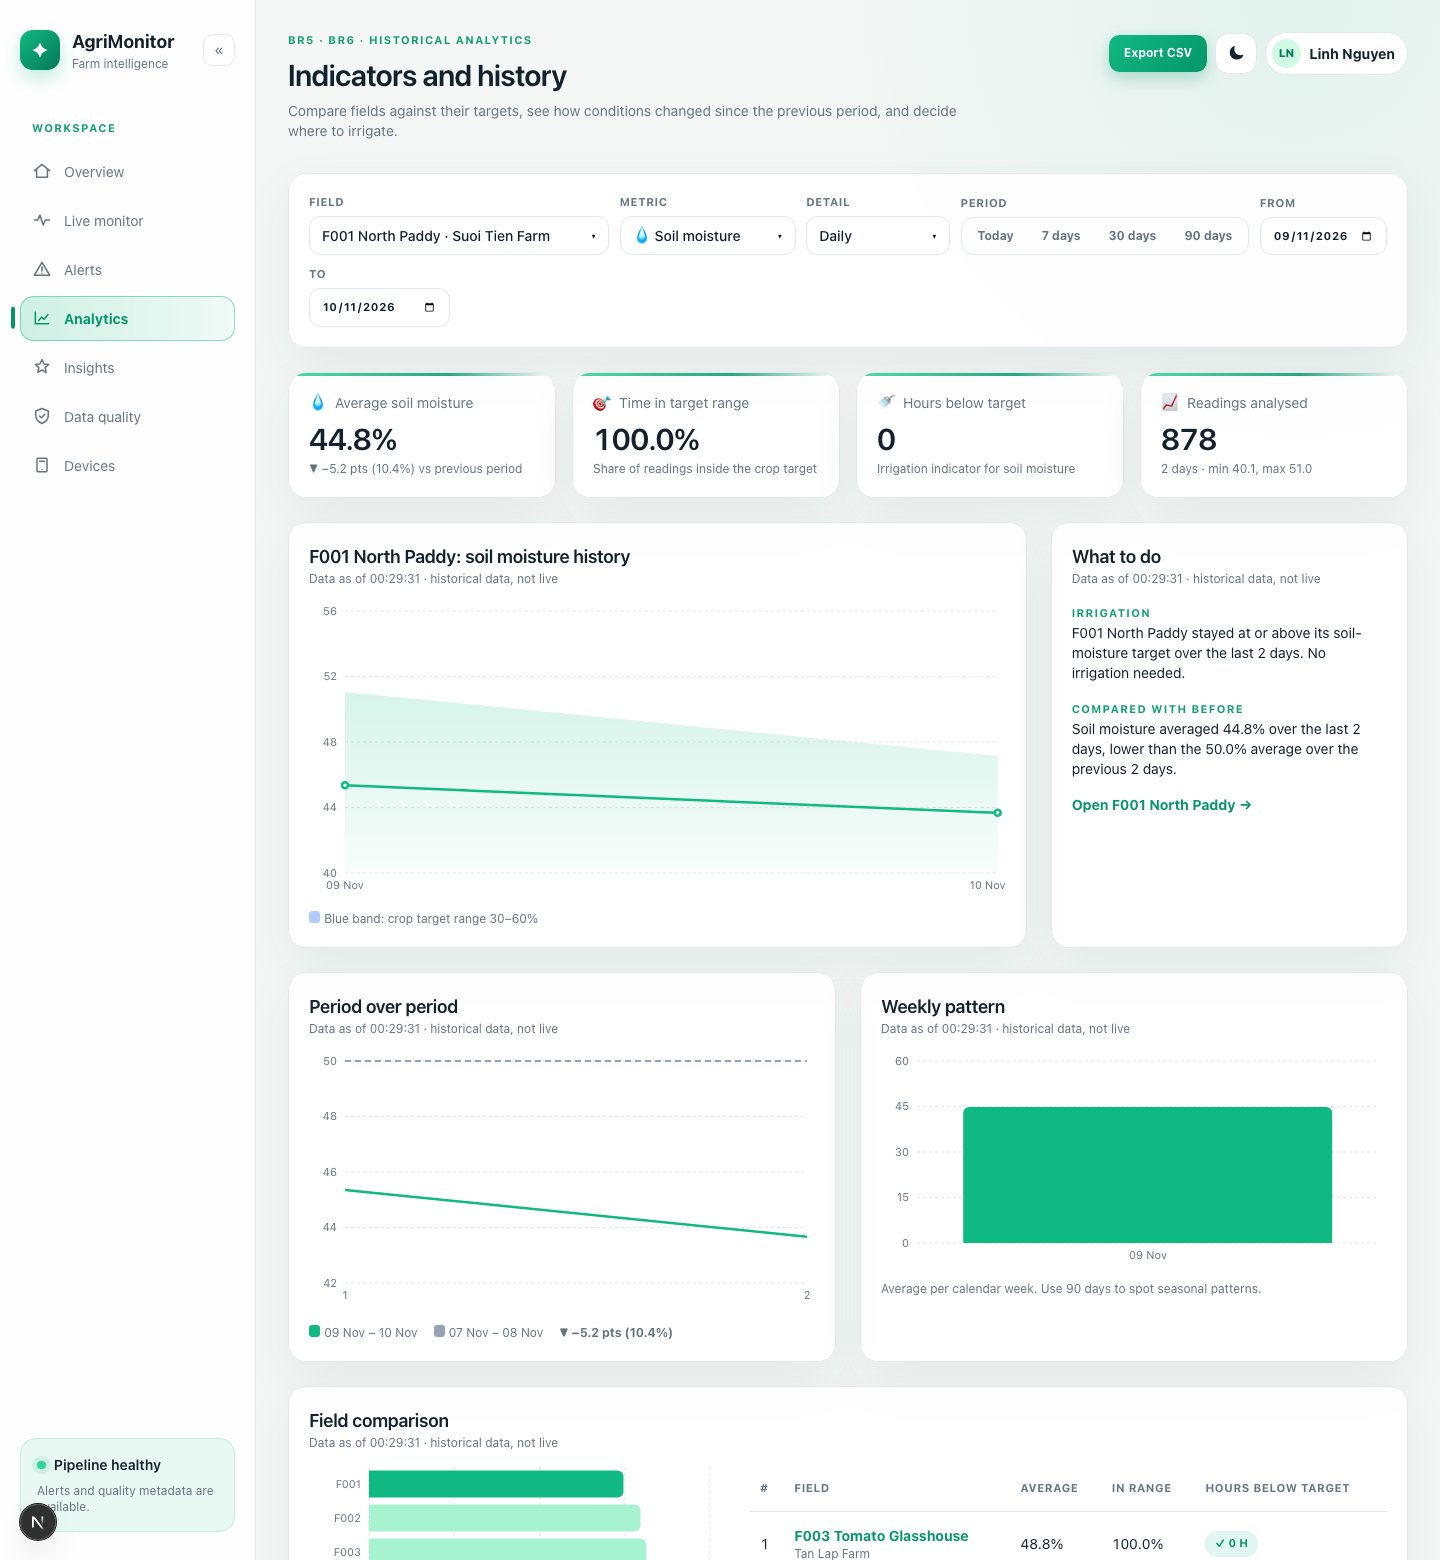
\includegraphics[width=0.95\linewidth]{analytics-period.png}
\caption{Trang Analytics: so sánh 9--10/11 với 7--8/11 của F001 (độ ẩm đất trung bình 44,8\% so với 50,0\%)}
\label{fig:4-br06-ui}
\end{figure}

\paragraph{Giới hạn của dữ liệu.} Bộ mô phỏng chỉ sinh dữ liệu trên một khoảng ngắn và thưa (nhiều ngày chỉ có một bản ghi), nên không có hai mùa vụ thật để so sánh và một số khoảng so sánh giai đoạn không có dữ liệu ở giai đoạn trước (giao diện hiển thị ``no data'' thay vì số 0). Tiêu chí về mùa vụ vì vậy chỉ chứng minh được \emph{cơ chế}: tổng hợp theo tuần và so sánh hai khoảng cùng độ dài. Báo cáo ghi nhận đây là một hạn chế (Mục~\ref{sec:5-discussion}). Nếu cần minh họa tốt hơn, có thể nạp trước một lịch sử mô phỏng dài hơn trước khi dựng gold, nhưng đó vẫn là dữ liệu mô phỏng chứ không phải mùa vụ thật.

\paragraph{Kịch bản minh họa.} Nhà phân tích chọn F001, so hai ngày gần nhất với hai ngày trước đó, và thấy độ ẩm đất trung bình giảm 5,2 điểm phần trăm. Họ chạy truy vấn time travel trên bảng \code{field\_indicators} tại snapshot đã ghi lúc xuất báo cáo và nhận lại đúng số liệu cũ, kể cả khi dữ liệu và khoảng mục tiêu đã đổi sau đó.
